\section{Resultados}
\subsection{Discos de Magdeburg}

%TODO: formatar e, talvez mudar algumas coisas de seção

Durante o experimento, os hemisférios foram encaixados e alinhados (\cref{foto hemisferios}). Posteriormente, ao serem puxados em direções opostas (por forças de tração) eles não se separaram nem apresentaram deformação notável, indicando que tais forças não superaram aquelas que os uniam. Tal resultado pode ser explicado pelo fato de que entre discos ocorre um vácuo (sem possibilidade de entrada de ar), logo por fora há a pressão atmosférica pressionando-os, sendo que ela não é contrabalanceada por uma pressão interna, sendo essa segunda mínima.

\begin{figure}[H]
    \centering
    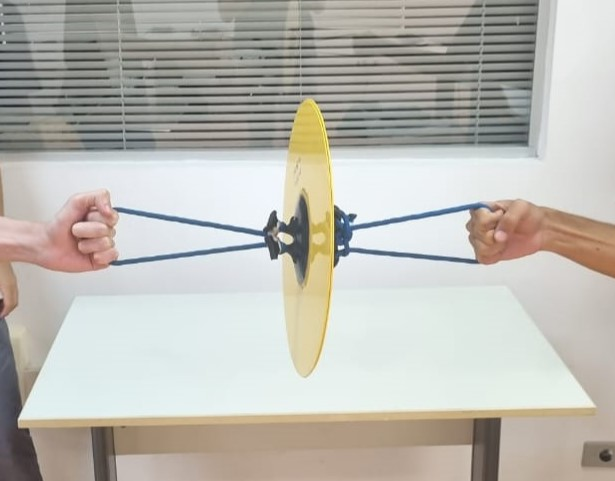
\includegraphics[width=0.5\textwidth]{fig/Cortada.jpeg}
    \caption{Hemisférios sob tração}
    \label{foto hemisferios}
\end{figure}
Foi feito também um diagrama (\cref{esquema hemisférios}) das forças que atuam sobre um dos hemisférios no eixo horizontal (em que é feita a tração).

\begin{figure}[H]
    \centering
    \includegraphics[width=0.5\textwidth]{fig/Diagrama de forças hemisferio.png}
    \caption{Esquema dos hemisférios sob tração. Em que Fa é a força feita pela pressão atmosférica; Fh2 é a força aplicada pelo segundo hemisfério sobre o analisado, por ser pressionado pela pressão atmosférica; T é tração feita pelos estudantes que puxavam os hemisférios.}
    \label{esquema hemisférios}
\end{figure}

Como o sistema encontrava-se em equilíbrio (estático), pode-se concluir que, em módulo, Fa = Fh2 + T. Além disso, dado que a pressão atmosférica é constante e a área dos discos também (logo Fa é fixa), pode-se concluir que Fh2 deve reduzir proporcionalmente ao aumento da tensão T. Por fim, para separar os discos, seria necessária uma tração, em cada lado (se iguais) superior à força atmosférica:

\begin{align*}
    Fa = \text{pressão} \times \text{área}\\
    \text{Área*} = 962 cm^2 = 9,62 \times 10^{-2}m^2\\
    \text{Pressão atmosférica*:} 9,235 \times 10^4 Pa = N/m^2\\
    Fa = (9,235 \times 10^4) * (9,62 \times 10^{-2}) = 8,88 \times 10^3 N  
\end{align*}

	Logo, a força de cada lado para separar os discos seria de \(8,88 \times 10^3 N\), aproximadamente equivalente a \(8,71 \times 10^4\) kg.
 
	*Foi utilizada a pressão atmosférica medida pelo Instituto de Astronomia, Geofísica e Ciências Atmosféricas da Universidade de São Paulo %TODO: citar a ref de baixo aqui 

    %TODO: Por isso aqui como referência(de 923.5 hPa em 30/3/2025, http://www.estacao.iag.usp.br/index.php).
    
	Cálculo de erro: a área foi calculada a partir do diâmetro do hemisfério, de 350cm (logo temos um erro associado de \(\pm5cm = \pm5\times10^{-2}m\), sendo que o valor foi elevado ao quadrado). Além disso, podemos estimar o erro da medição de pressão como \(\pm 10\) Pa.

	Por propagação de incerteza (tome R como raio e P como pressão):
    
Erro =

\begin{align*}
\sqrt{\left( \frac{\partial }{\partial R} R^{2}\pi P \times\sigma R \right)^{2} + \left( \frac{\partial }{\partial P} R^{2}\pi P \times \sigma P \right)^{2}} =
\sqrt{\left( 2 \times 3,5\pi 92350 \times 0,05 \right)^{2} + \left(3,5^{2}\pi \times 10 \right)^{2}} \cong 
\pm101544  \cong  1 \times 10^5
\end{align*}

Pode-se notar que o erro calculado é superior ao próprio resultado obtido, o que indica a necessidade de uma possível revisão na forma de cálculo de erro utilizada, ou uma forte imprecisão do cálculo devido ao uso de grandezas muito discrepentes (o próprio erro da pressão era superior ao raio, o que pode ter causado tal grande incerteza).

\subsection{Frasco com membrana}

Após análise com o software Traker, obtemos a \cref{copo.png}. Veja

\begin{figure}[H]
    \centering
    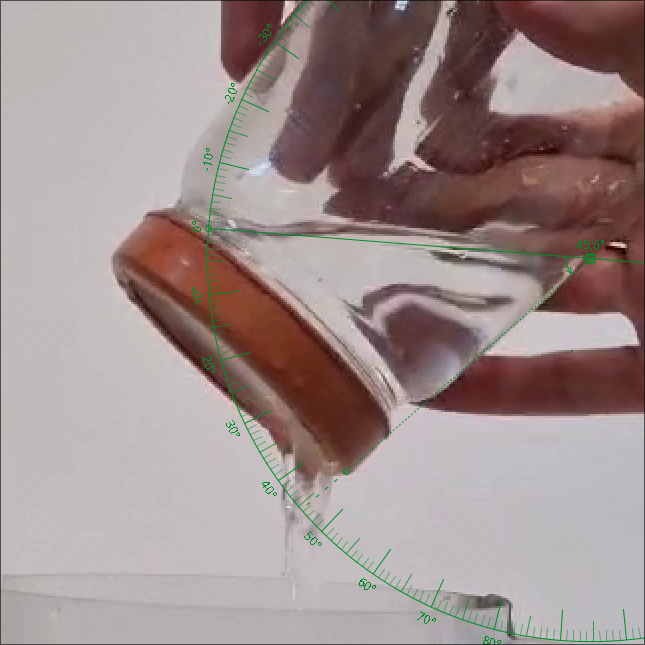
\includegraphics[width=.5\linewidth]{fig/copo.png}
    \caption{Ângulo de inclinação do copo para equilíbrio de pressões}
    \label{copo.png}
\end{figure}

Note a inclinação do frasco em relação ao nível da água, em torno de \( 45,6 \)° .

%
%
%
\subsection{Manõmetros}

Para este experimento, vamos avaliar os valores da seguinte maneira:
\begin{enumerate}
    \item Vamos nomear de Extremidade da Atmosfera, E. Atm, a ponta do tubo em U aberta que está aberta;
    \item Vamos nomear de Extremidade do Recipiente, E. Recip, a ponta do tubo em U na qual se conecta o cano móvel a ser submerso no recipiente;
    \item Vamos nomear de Extremidade Livre, E. Livre, a ponta de vidro de diâmetro maior do cano móvel que submergimos no líquido.
\end{enumerate}

Dessa forma, os valores obtidos estão sintetizados na \cref{tab_man}

\begin{table}[H]
    \centering
    \begin{tabular}{c | c | c}
        \hline
        \textbf{E. Livre (cm \(\pm 0,5\))} & \textbf{E. Atm (cm\(\pm 0,5\))} & \textbf{E. Recip (cm \(\pm0,5\))}\\
        \hline
        11,0 & 12,2 & 12,2\\
        \hline
        16,0 & 14,5 & 11,1\\
        \hline
        21,0 & 16,2 & 9,0\\
        \hline
    \end{tabular}
    \caption{Valores mensurados com o manômetro de tubo aberto}
    \label{tab_man}
\end{table}

\subsection{Densidade do líquido}
Definindo a linha paralela à separação da fase de água com a fase do líquido misterioso como ponto de altura \(h = 0\), podemos determinar a altura em que a água fica exposta ao ar como \(h_w = \qty{0,123}{m}\) e a altura na qual o líquido misterioso fica exposto ao ar como \(h_l = \qty{0,153}{m}\). Com esses dados, a lei de Stevin nos permite calcular a densidade do líquido misterioso:
\begin{align*}
    \rho_l \cdot h_l &= \rho_w \cdot h_w\\
    \rho_l &= \frac{\rho_w \cdot h_w}{h_l}\\
    \rho_l &= \frac{966,5 \cdot 0,123}{0,153} =  
\end{align*}
\subsection{Manõmetros}
